\documentclass{ximera}
\title{Newton's Methods}
\begin{abstract}
\end{abstract}
\begin{document}
\maketitle
\section{Introduction}
\begin{dialogue}
\item[Dylan] I'm so tired of having to solve roots by hand. It's a real drag.
\item[Julia] Yeah, some of these roots are rough. I wish there was a better way!
\item[James] There's always a better way!
\item[Dylan and Julia] Show us!!!
\item[James] Maybe you've heard of Sir Isaac Newton? He got tired of solving roots too, and made a whole method to approximate them!
\item[Dylan] Wow! I'm just like him except worse in every way!
\end{dialogue}
Newton's Method is a system of approximating roots of polynomials by using tangent lines from an initial estimate. While this method is extremely accurate when used properly, it is possible to have a very inaccurate estimate when used improperly.
\section{Guided Example}
In the following figure we have an initial guess $x_{0}$, then we have the blue tangent line with respect to the point $x_{0}$
\begin{image}
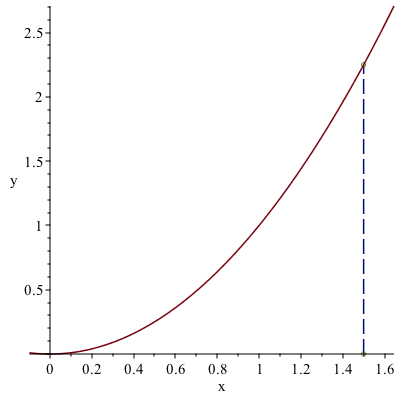
\includegraphics{NewtonMethod}
\end{image}
\begin{question}

What is the slope, in general, for the tangent line of $y=f(x)$ at $x_{0}$?

\begin{multipleChoice}
\choice[correct]{$f'(x_0)$}
\choice{$f'(x)$}
\choice{$f(x)$}
\choice{$f(f(x))$}
\end{multipleChoice}

What is the equation of the tangent line for the point $(x_{0},f(x_{0})$? Please answer in slope-intercept form.

\begin{multipleChoice}
\choice{$y=f(x) \cdot x + b$}
\choice[correct]{$y = f'(x_0)\cdot x_0+b$}
\choice{$y = f'(x) \cdot b + x_0$}
\choice{$y = f'(x) \cdot b + f(x)$}
\end{multipleChoice}

How would you use the tangent line you found above to estimate the value of $x_{1}$?

\begin{freeResponse}
\end{freeResponse}

\end{question}
\section{On Your Own}
\begin{question}
Consider the function $f(x) = x^2-1$.
\[
\graph{x^2-1}
\]

Find the equation of the tangent line at an initial estimate of $x_0=3$.

$y = \answer{}$

Plot the tangent line and function on the same axes. Does the x-intercept of the tangent line seem more or less accurate than your initial estimate?

\begin{multipleChoice}
\choice[correct]{More Accurate}
\choice{Less Accurate}
\end{multipleChoice}

What is the x-intercept of the tangent line?

$\answer{I don't know}$

Continue this process until the x-intercepts change by less than .0001 on each iteration. How many iterations did this take?

$\answer{}$
\end{question}
\begin{question}
Consider the function $g(x) = x^3-4x^2-1$.
\[
\graph{x^3-4x^2-1}
\]
Explain why the function has only one solution with the help of a graph.
\[
\graph{}
\]
\begin{freeResponse}
\end{freeResponse}
Using $g(x)$ from the previous problem, use an initial guess of 2. After 5 iterations, what result do you get?
$\answer{A really bad one}$

Why is it important to use caution with Newton's method?
\begin{freeResponse}
\end{freeResponse}
\end{question}

\begin{question}
Consider the function $h(x) = 4x^3 - 12x^2 + 2x + 1$.
\[
\graph[xmin=-6,xmax=6,ymin=-15,ymax=7,height=400]{4x^3 - 12x^2 + 2x + 1}
\]

Use an initial guess of $x=3$ to estimate a root of $h(x)$. What do you find?

$\answer{}$

Look at the graph, and attempt to estimate another root using $x = 0$. Did you find the root to the right or the left of this point?

\begin{multipleChoice}
\choice[correct]{Left}
\choice{Right}
\end{multipleChoice}

Increment the initial guess by $0.02$ and use Newton's method until you find the other root. What value of $x$ is the first to work?
$\answer{}$
\end{question}

\section{In Summary}
\begin{dialogue}
\item[Julia] Wow! Newton's Method is awesome!
\item[Dylan] Yeah, it's way more accurate than just guessing! If you're too far off on that initial guess though...
\item[James] Things can go downhill quickly. While Newton's Method can be handy, it's important to remember how important an accurate initial estimate is!
\item[Dylan and Julia] Thanks James!
\end{dialogue}
\end{document}